\section{Introducción}

\textbf{La productividad importa porque puede sostener mejores remuneraciones laborales, pero esa relación no es automática.} Un departamento puede producir mucho por trabajador y, aun así, no traducir esa productividad en remuneraciones proporcionalmente altas. También puede ocurrir lo contrario: algunos departamentos pueden mostrar remuneraciones relativamente altas para su nivel de producción por trabajador.

\textbf{Este informe analiza la relación entre productividad y remuneración laboral en los departamentos de Colombia.} El ejercicio combina el PIB departamental del DANE con ocupados, horas trabajadas e ingresos laborales de la GEIH. El objetivo no es establecer una relación causal, sino describir hasta qué punto los departamentos más productivos son también los que mejor remuneran el trabajo.

\textbf{La pregunta es relevante para la agenda de productividad.} Si la productividad crece, pero no se traduce en mejores remuneraciones, el vínculo entre crecimiento económico y bienestar laboral se debilita. Si, además, esa relación cambia entre territorios, la agenda de productividad debe mirar no solo cuánto produce cada departamento, sino también cómo se organiza su mercado laboral.

\textbf{El informe está organizado en seis secciones, incluyendo esta introducción.} La sección 2 presenta la metodología. La sección 3 compara los niveles de productividad y remuneración. La sección 4 analiza los departamentos que se apartan de la relación promedio entre ambas variables. La sección 5 compara el crecimiento de la productividad y de la remuneración. La sección 6 presenta conclusiones.

\section{Metodología}

\textbf{La medición combina cuentas nacionales departamentales y microdatos de la GEIH.} La productividad se calcula usando el PIB departamental real del DANE, expresado en pesos constantes de 2015, y el número de ocupados de la GEIH. La remuneración laboral se calcula con el ingreso laboral por hora, las horas trabajadas y el factor de expansión de la encuesta.

\textbf{La comparación principal se hace entre PIB por trabajador y remuneración por trabajador.} El PIB por trabajador divide el PIB real departamental entre el número anual de ocupados. La remuneración por trabajador divide la remuneración laboral mensual total observada entre ocupados con ingreso y horas válidas por el número total de ocupados del departamento. Esta construcción mantiene un denominador comparable para ambas variables.

\textbf{El informe se concentra en 24 departamentos comparables durante todo el periodo.} Para evitar imputaciones o cambios artificiales en la cobertura, se excluyen San Andrés y Providencia y los departamentos de la Amazonía y la Orinoquía que no hacen parte del panel comparable de la GEIH desde 2010. Bogotá D.C. se trata como departamento porque así aparece en las cuentas nacionales departamentales.

\textbf{El periodo de análisis es 2010--2024pr y se excluye 2020.} El año 2020 se excluye para mantener consistencia con los informes anteriores de la serie. Las tasas de crecimiento reportadas son tasas anualizadas entre 2010 y 2024pr.

\section{Productividad y remuneración en niveles}

\textbf{Los departamentos más productivos tienden a tener mayores remuneraciones, pero la relación no es perfecta.} El Cuadro \ref{tab:pib_geih_productividad_departamento_remuneracion} compara el ranking departamental de PIB por trabajador y remuneración por trabajador. Bogotá D.C. ocupa el primer lugar en ambas medidas, pero hay diferencias importantes en el resto de la distribución.

\begin{table}[H]
\centering
\caption{Ranking departamental de PIB por trabajador y remuneraci\'on por trabajador, 2024pr}
\label{tab:pib_geih_productividad_departamento_remuneracion}
\scriptsize
\begin{tabular}{lrrrrr}
\toprule
Departamento & PIB/trab. 2024pr & Puesto & Rem./trab. 2024 & Puesto & Dif. puestos \\
\midrule
Bogotá D.C. & 67,4 & 1 & 2,95 & 1 & +0 \\
Meta & 63,1 & 2 & 1,83 & 4 & +2 \\
Santander & 62,0 & 3 & 1,80 & 6 & +3 \\
Valle del Cauca & 54,5 & 4 & 1,79 & 7 & +3 \\
Antioquia & 47,7 & 5 & 2,12 & 2 & -3 \\
Boyacá & 47,5 & 6 & 1,49 & 13 & +7 \\
Bolívar & 45,1 & 7 & 1,33 & 16 & +9 \\
Cundinamarca & 40,4 & 8 & 1,79 & 8 & +0 \\
Tolima & 40,0 & 9 & 1,50 & 11 & +2 \\
Risaralda & 38,7 & 10 & 1,82 & 5 & -5 \\
Atlántico & 37,3 & 11 & 1,58 & 10 & -1 \\
Caldas & 36,6 & 12 & 1,85 & 3 & -9 \\
Quindío & 33,8 & 13 & 1,71 & 9 & -4 \\
Cesar & 32,6 & 14 & 1,26 & 17 & +3 \\
Huila & 31,6 & 15 & 1,36 & 15 & +0 \\
Chocó & 28,6 & 16 & 1,16 & 18 & +2 \\
Cauca & 26,6 & 17 & 1,06 & 20 & +3 \\
Caquetá & 24,9 & 18 & 1,47 & 14 & -4 \\
La Guajira & 24,8 & 19 & 0,89 & 24 & +5 \\
Norte de Santander & 24,3 & 20 & 1,49 & 12 & -8 \\
Magdalena & 23,9 & 21 & 1,15 & 19 & -2 \\
Córdoba & 22,0 & 22 & 1,04 & 22 & +0 \\
Sucre & 22,0 & 23 & 1,01 & 23 & +0 \\
Nariño & 17,8 & 24 & 1,06 & 21 & -3 \\
\bottomrule
\end{tabular}
\caption*{\footnotesize Nota: PIB por trabajador en millones de pesos constantes de 2015; remuneraci\'on por trabajador en millones de pesos constantes de 2025 al mes. La remuneraci\'on por trabajador se calcula como la remuneraci\'on laboral mensual total observada entre ocupados con ingreso horario positivo y horas v\'alidas, dividida por el n\'umero total de ocupados del departamento. La diferencia de puestos corresponde al puesto en remuneraci\'on menos el puesto en PIB por trabajador; un valor positivo indica que el departamento ocupa una posici\'on m\'as baja en remuneraci\'on que en productividad. Fuente: c\'alculos propios con DANE y GEIH.}
\end{table}

\textbf{La comparación de rankings muestra que productividad y remuneración no ordenan a los departamentos exactamente de la misma forma.} Caldas y Antioquia tienen una mejor posición relativa en remuneración que en PIB por trabajador. En sentido contrario, Meta, Santander, Bolívar, Boyacá y La Guajira tienen una posición más favorable en PIB por trabajador que en remuneración. Estas diferencias no significan que unos departamentos paguen demasiado y otros muy poco; muestran que la remuneración también depende de la composición sectorial, la informalidad, la calificación de los trabajadores y la estructura empresarial.

\begin{figure}[H]
  \centering
  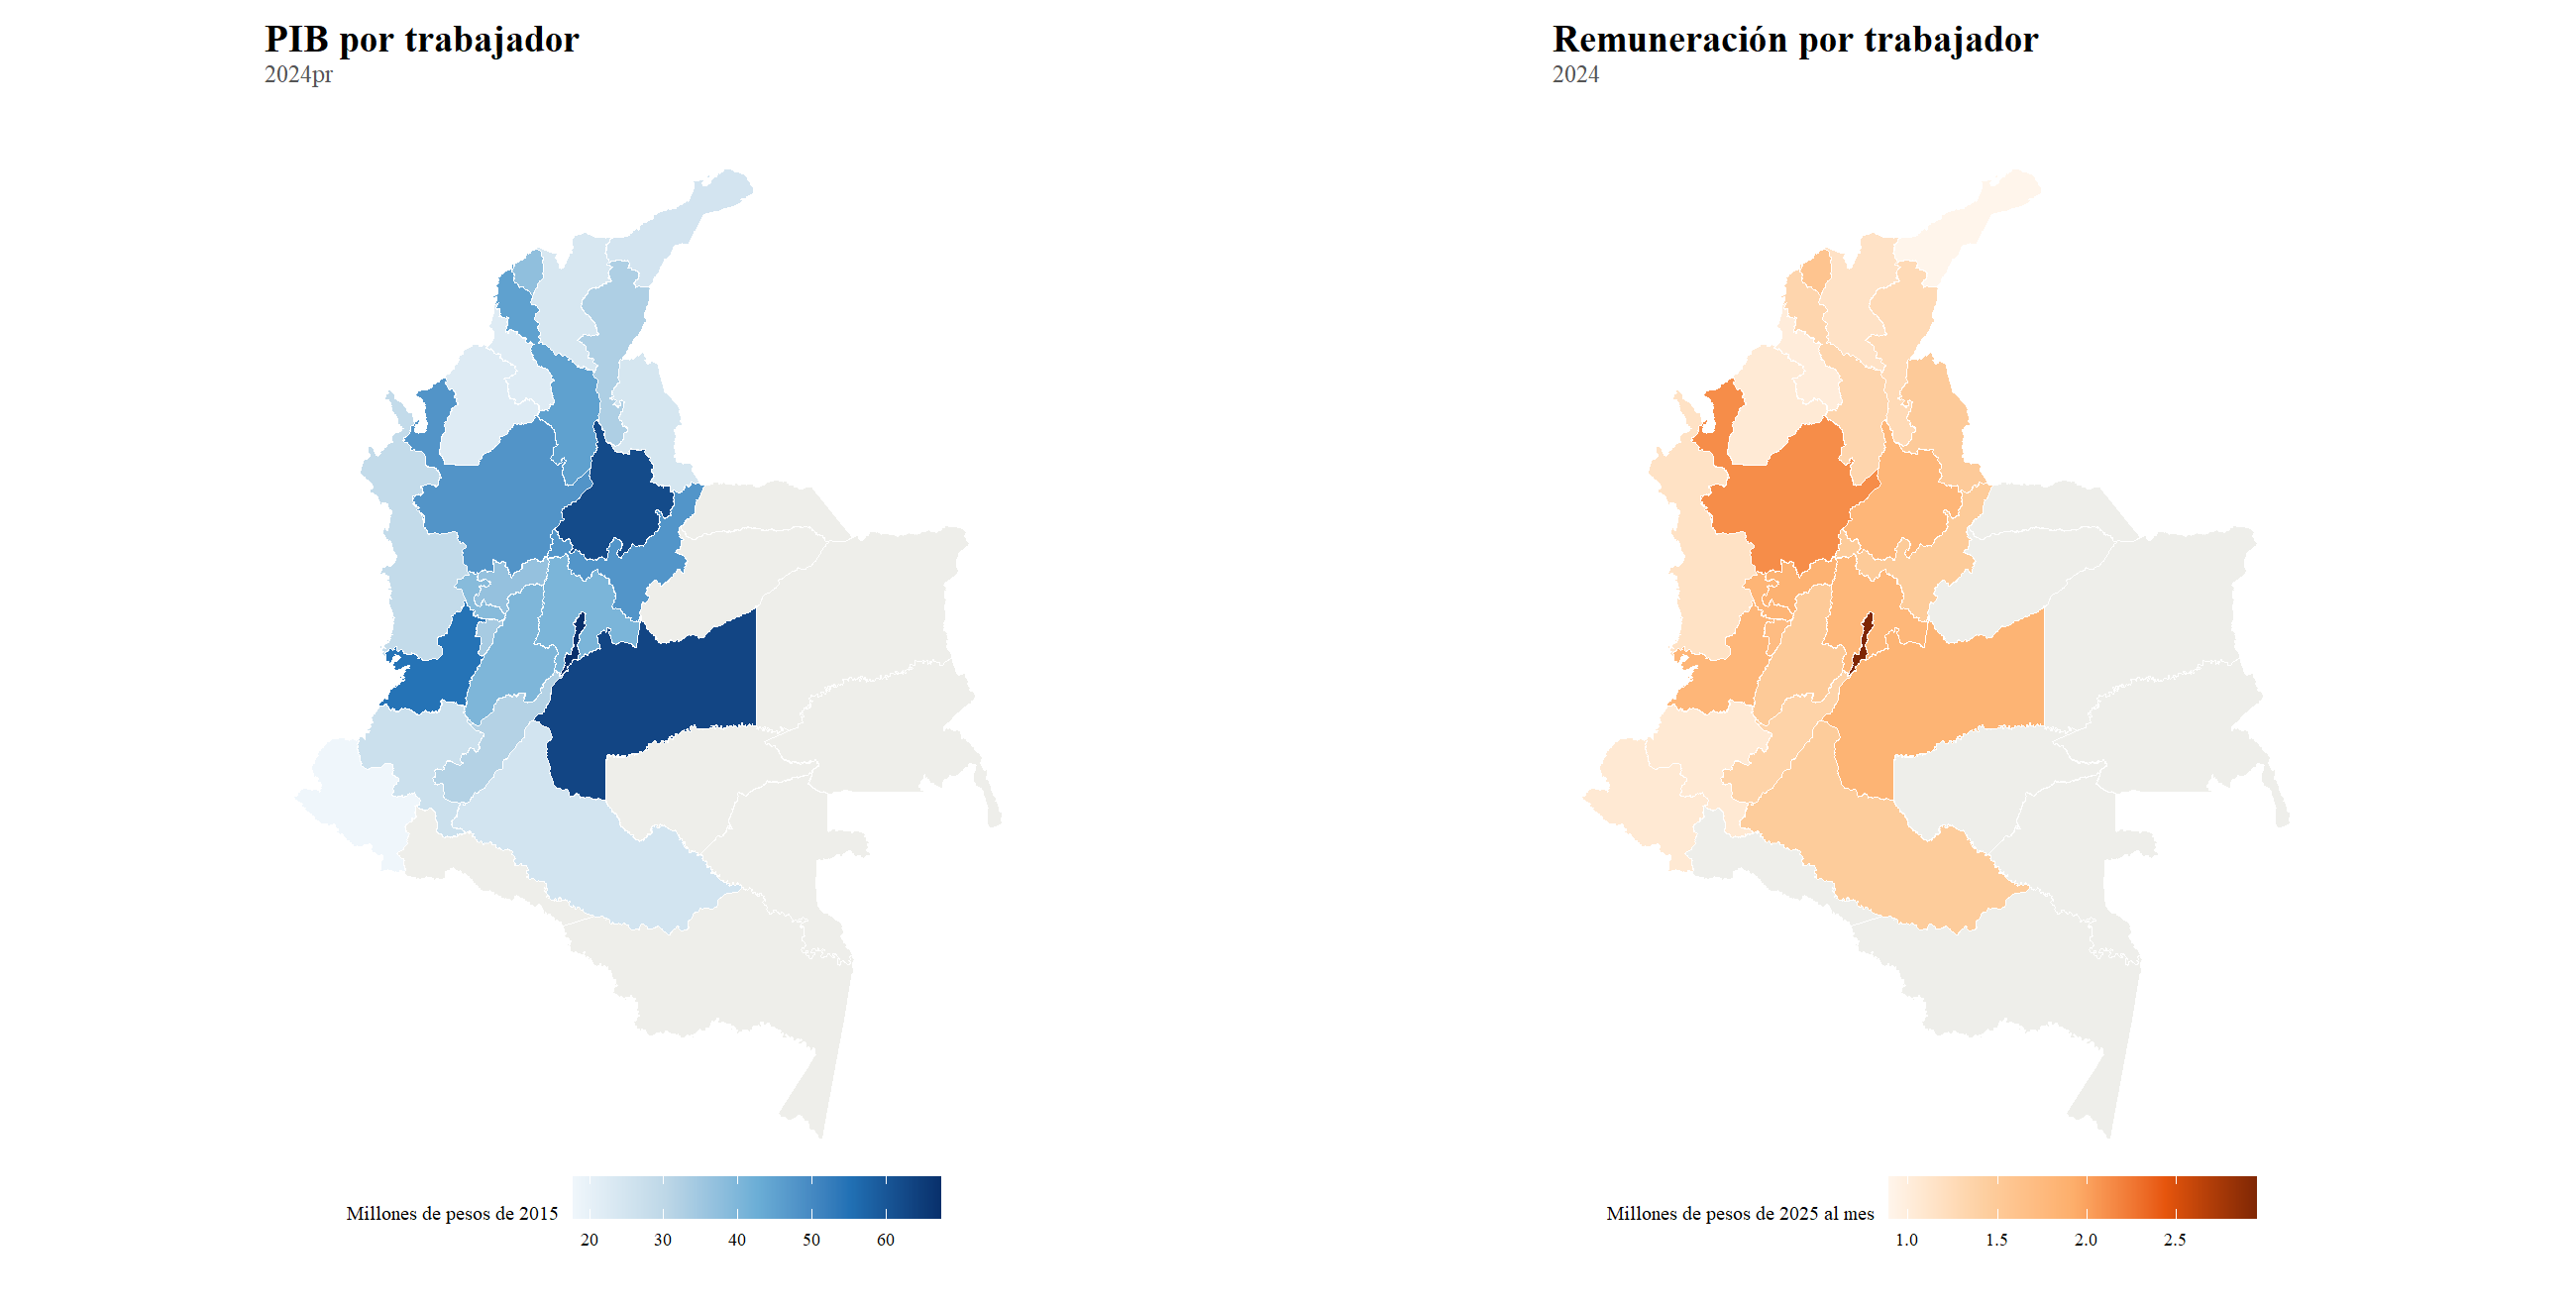
\includegraphics[width=\textwidth]{Paper/figures/fig_pib_geih_productividad_departamento_mapa_niveles.png}
  \caption{Mapa de niveles de PIB por trabajador y remuneración por trabajador, 2024}
  \label{fig:pib_geih_productividad_departamento_mapa_niveles}
  \caption*{\footnotesize Nota: la figura cubre los 24 departamentos comparables en la GEIH durante todo el periodo; los demás departamentos aparecen en gris. Fuente: cálculos propios con DANE y GEIH; geometría departamental de GADM.}
\end{figure}

\textbf{El mapa muestra que la geografía de la productividad y la geografía de la remuneración se parecen, pero no son idénticas.} Los tonos más oscuros de productividad se concentran en Bogotá D.C., Meta, Santander, Valle del Cauca y Antioquia, mientras que la remuneración por trabajador se concentra con más fuerza en Bogotá D.C. y Antioquia. La comparación visual refuerza el punto central del informe: producir más por trabajador y remunerar más al trabajador están relacionados, pero no son el mismo fenómeno.

\begin{figure}[H]
  \centering
  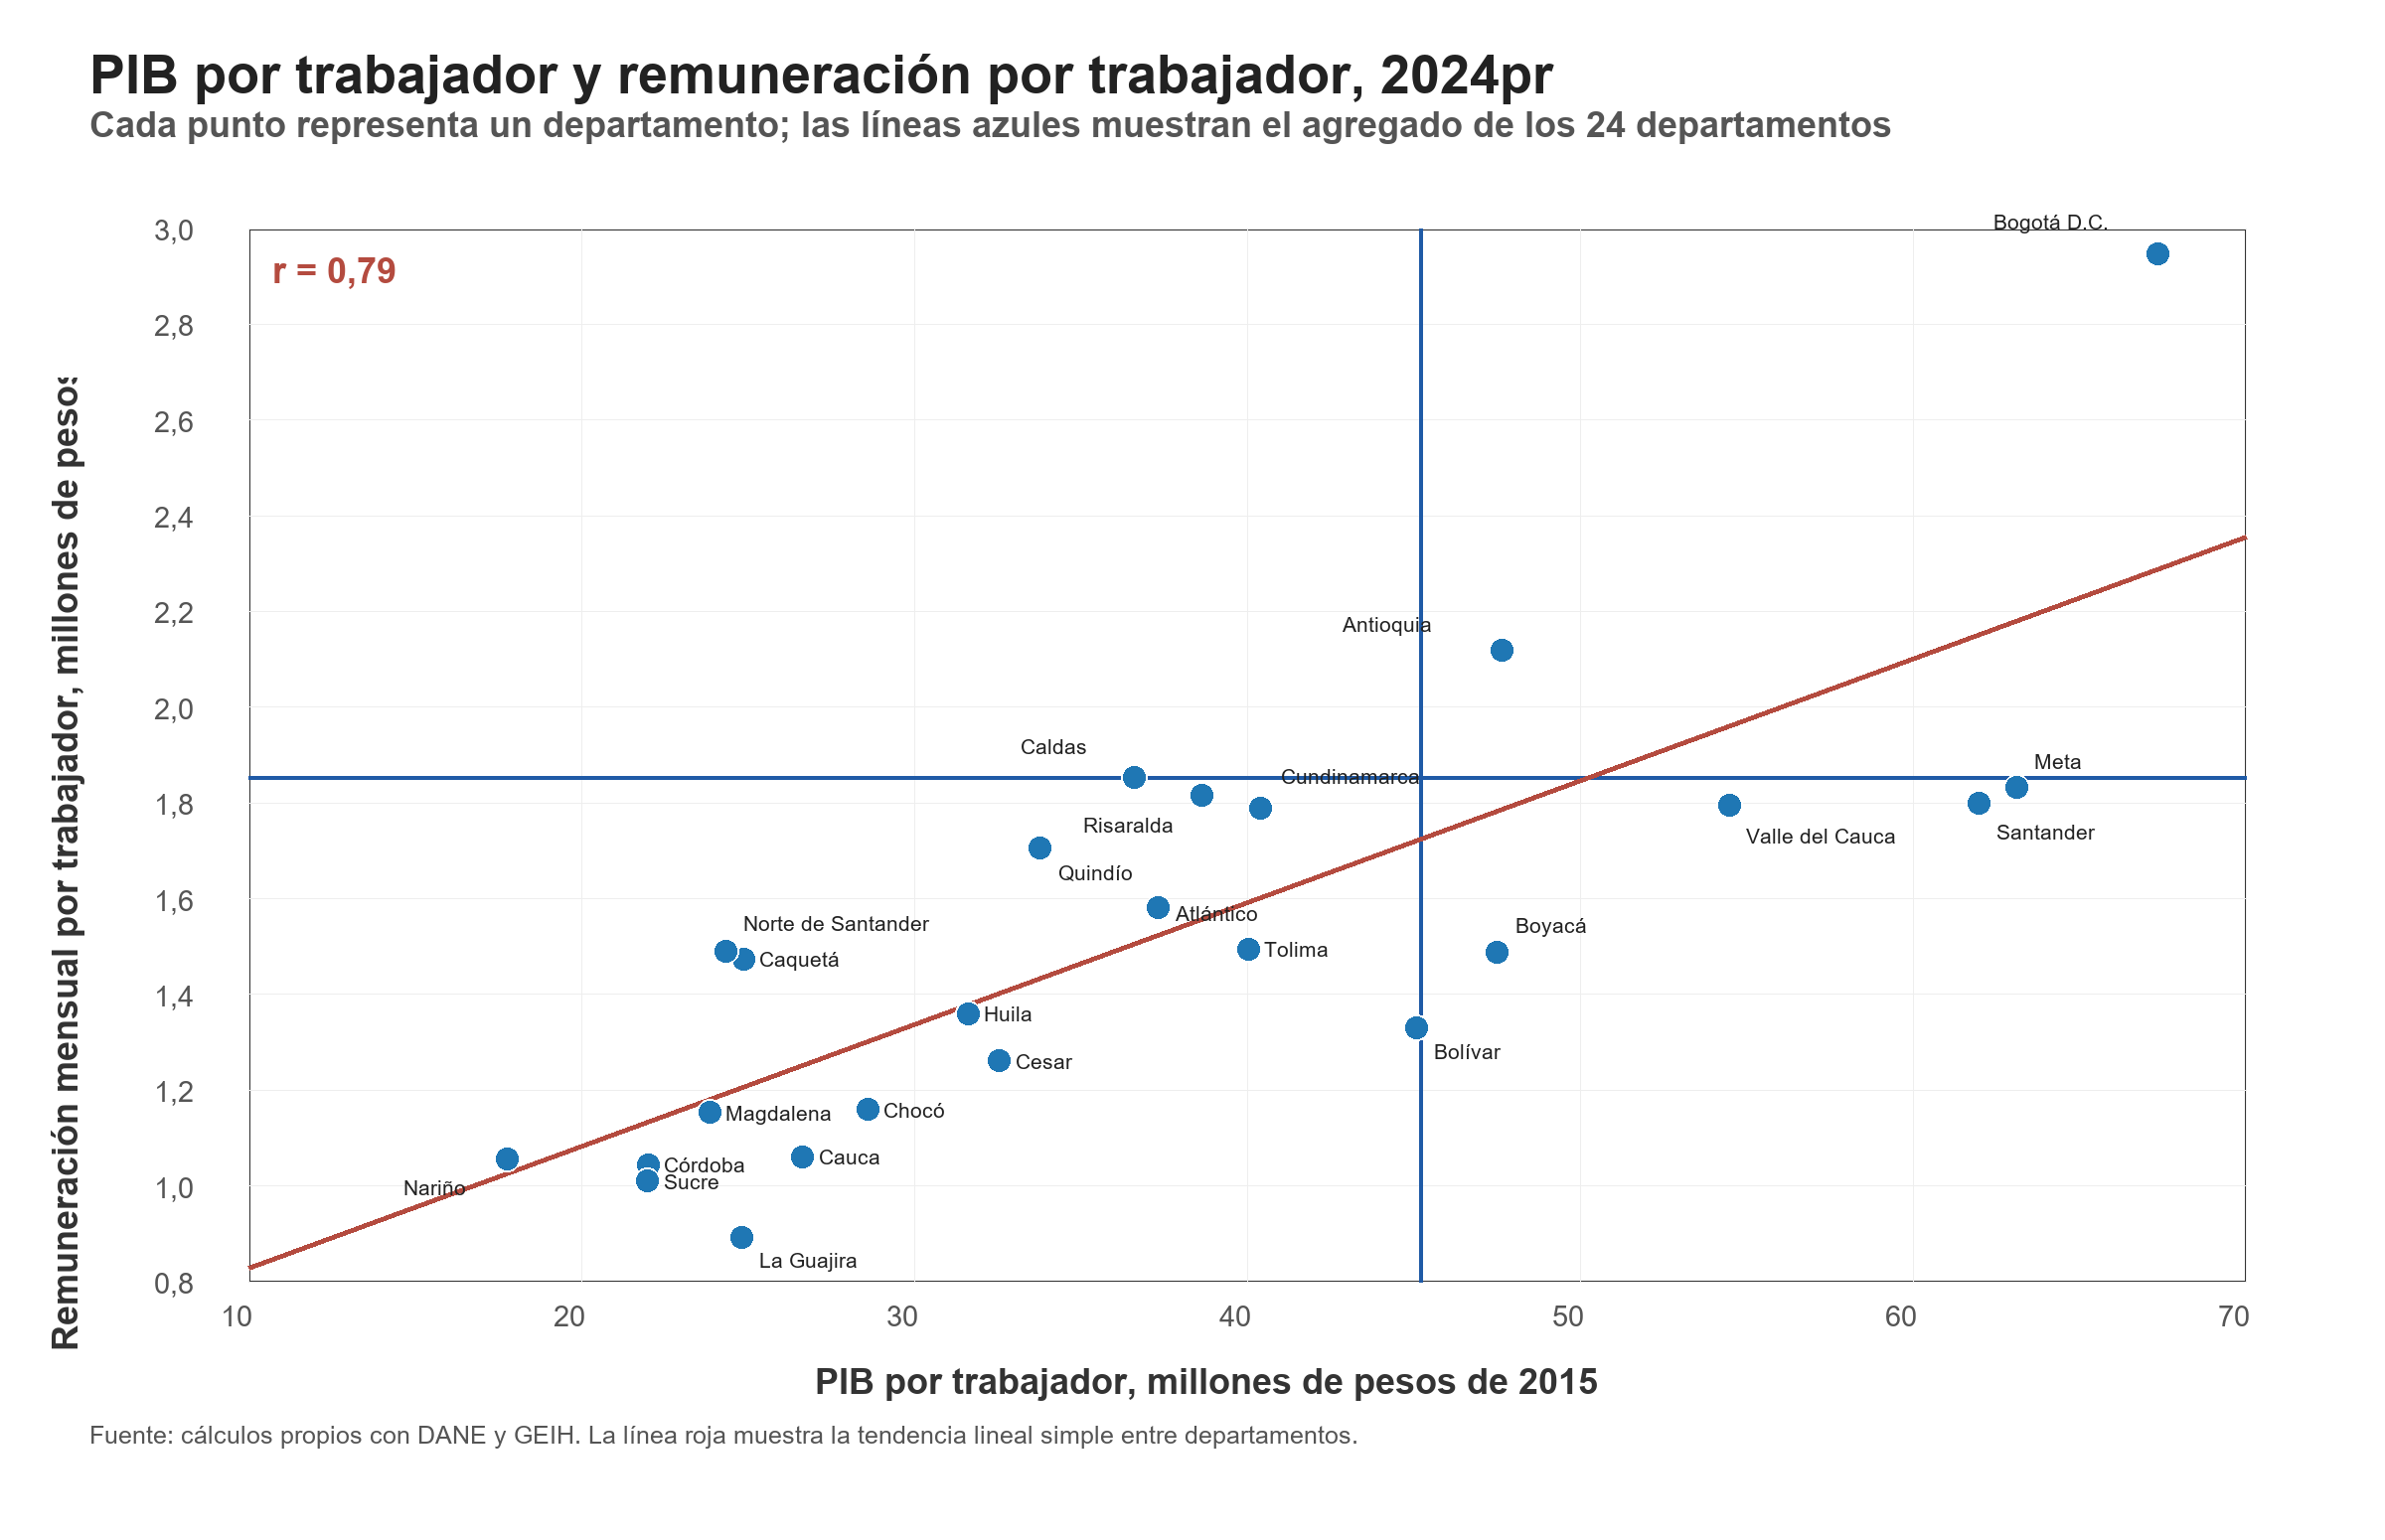
\includegraphics[width=\textwidth]{Paper/figures/fig_pib_geih_productividad_departamento_remuneracion.png}
  \caption{PIB por trabajador y remuneración por trabajador por departamento, 2024pr}
  \label{fig:pib_geih_productividad_departamento_remuneracion}
\end{figure}

\textbf{La Figura \ref{fig:pib_geih_productividad_departamento_remuneracion} muestra una asociación clara entre productividad y remuneración.} La correlación entre el PIB por trabajador y la remuneración por trabajador es cercana a 0,8 entre los 24 departamentos comparables. Sin embargo, la dispersión alrededor de la línea de tendencia confirma que los niveles de remuneración también reflejan otros factores territoriales y laborales.

\section{Departamentos por encima y por debajo de la relación promedio}

\textbf{Los departamentos más alejados de la recta son especialmente informativos.} Por encima de la relación promedio aparecen Bogotá D.C., Caldas, Antioquia, Norte de Santander, Quindío, Caquetá y Risaralda: para su nivel de PIB por trabajador, registran una remuneración por trabajador mayor a la que sugiere la tendencia entre departamentos. Por debajo de la recta aparecen Bolívar, Santander, Meta, La Guajira y Boyacá: para su nivel de PIB por trabajador, registran una remuneración menor a la que sugiere la relación promedio.

\begin{figure}[H]
  \centering
  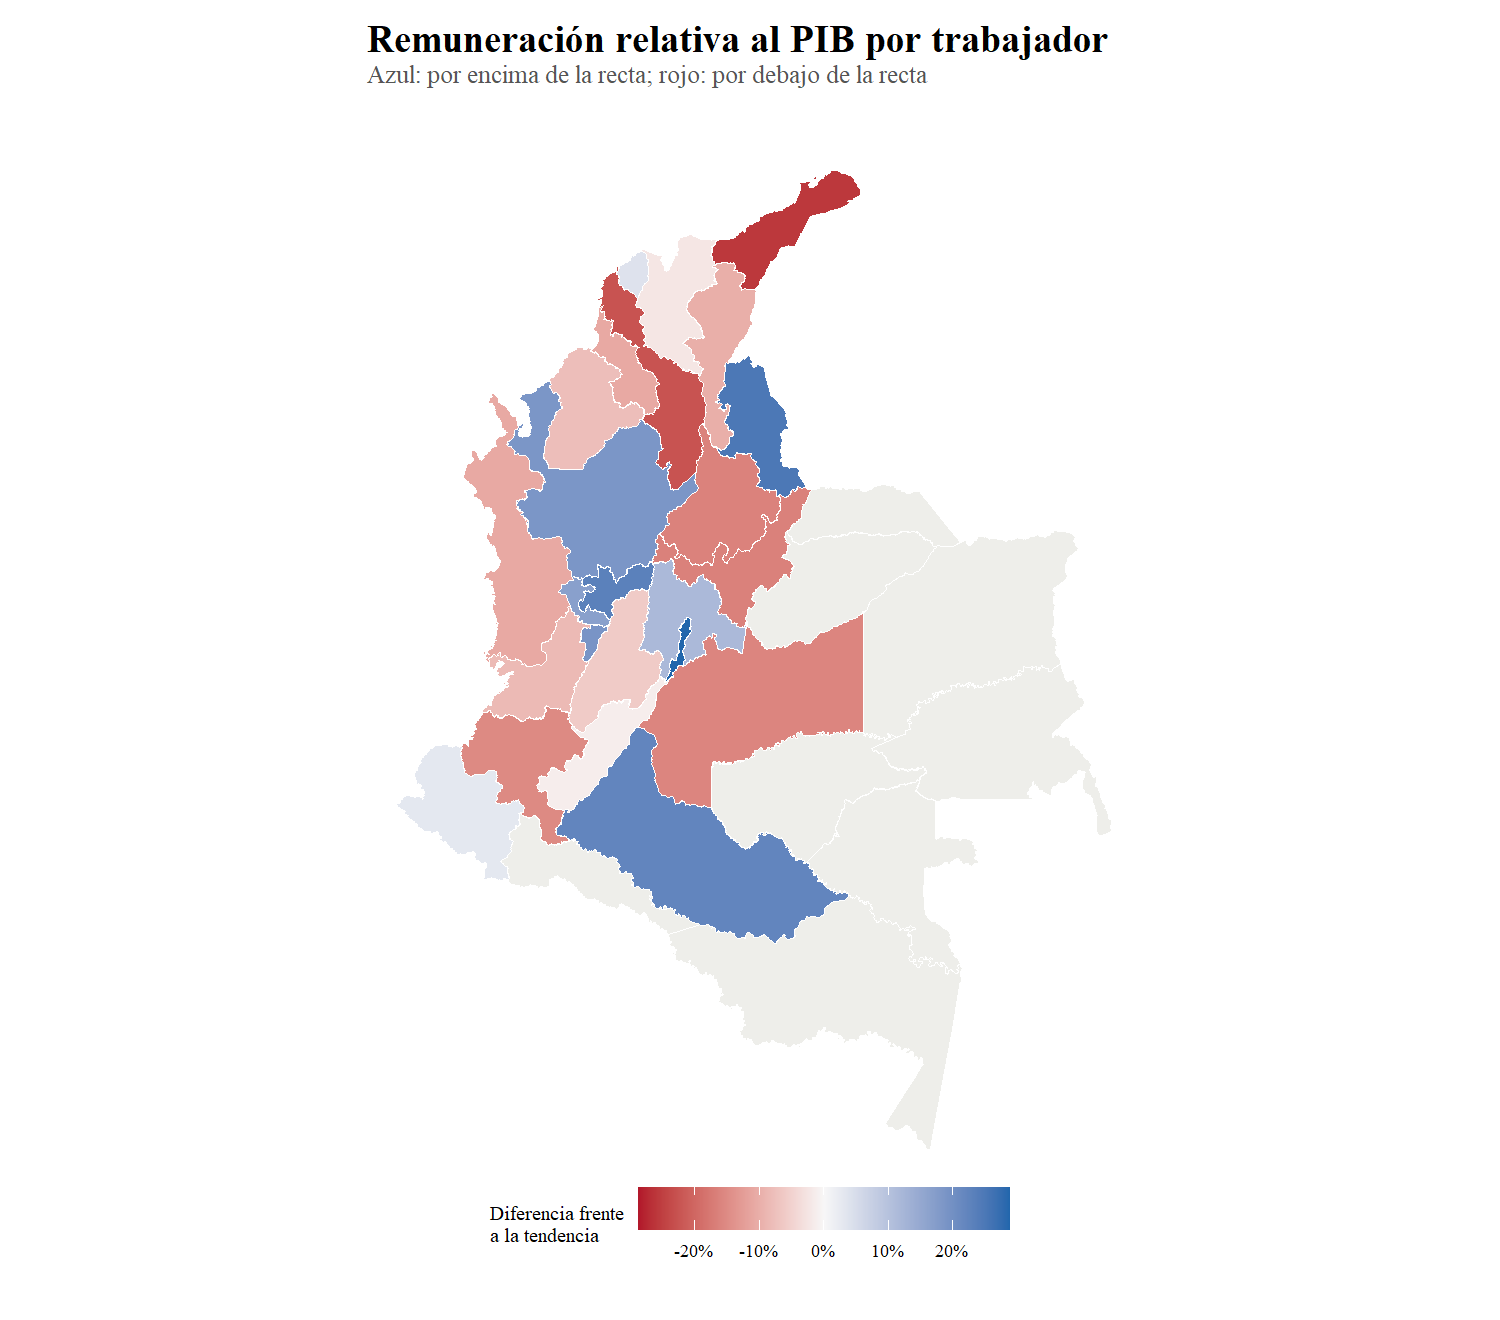
\includegraphics[width=0.82\textwidth]{Paper/figures/fig_pib_geih_productividad_departamento_mapa_residuos.png}
  \caption{Mapa de remuneración relativa al PIB por trabajador, 2024}
  \label{fig:pib_geih_productividad_departamento_mapa_residuos}
  \caption*{\footnotesize Nota: el color muestra la distancia porcentual entre la remuneración observada por trabajador y la remuneración predicha por la tendencia lineal entre PIB por trabajador y remuneración por trabajador. Azul indica remuneraciones por encima de la tendencia; rojo indica remuneraciones por debajo. Los departamentos no comparables aparecen en gris. Fuente: cálculos propios con DANE y GEIH; geometría departamental de GADM.}
\end{figure}

\textbf{El mapa de residuales muestra dónde la remuneración se aparta más de la relación promedio con la productividad.} Bogotá D.C., Caldas, Antioquia, Norte de Santander, Quindío, Caquetá y Risaralda aparecen en tonos azules porque registran remuneraciones superiores a las que sugiere su nivel de PIB por trabajador. En cambio, Bolívar, Santander, Meta, La Guajira y Boyacá aparecen en tonos rojos porque registran remuneraciones inferiores a las sugeridas por la tendencia. Esta lectura complementa el diagrama de dispersión porque muestra que esas diferencias no son solo casos aislados, sino patrones territoriales visibles.

\textbf{La interpretación debe ser prudente.} El ejercicio no permite afirmar que unos departamentos paguen demasiado y otros muy poco. Más bien señala que la conexión entre productividad y remuneración pasa por la estructura productiva y laboral de cada territorio. En particular, los casos de Meta, Santander y Bolívar son importantes porque combinan niveles altos de PIB por trabajador con remuneraciones relativamente más bajas frente a la tendencia.

\section{Crecimiento de productividad y crecimiento de remuneración}

\textbf{El crecimiento de la remuneración y el crecimiento del PIB por trabajador están relacionados, pero menos que sus niveles.} El Cuadro \ref{tab:pib_geih_productividad_departamento_remuneracion_crecimientos} compara las tasas de crecimiento anualizadas de ambas variables. La correlación entre ambas tasas de crecimiento es cercana a 0,45, menor que la correlación observada en niveles.

\begin{table}[H]
\centering
\caption{Crecimiento departamental de remuneraci\'on y PIB por trabajador, 2010--2024pr}
\label{tab:pib_geih_productividad_departamento_remuneracion_crecimientos}
\scriptsize
\begin{tabular}{lrrrrr}
\toprule
Departamento & Crec. rem./trab. & Puesto & Crec. PIB/trab. & Puesto & Dif. puestos \\
\midrule
Risaralda & 2,83\% & 1 & 3,14\% & 3 & -2 \\
Cundinamarca & 2,39\% & 2 & -0,32\% & 23 & -21 \\
Caldas & 2,30\% & 3 & 2,14\% & 6 & -3 \\
Bogotá D.C. & 1,90\% & 4 & 1,98\% & 8 & -4 \\
Boyacá & 1,66\% & 5 & 1,16\% & 15 & -10 \\
Antioquia & 1,65\% & 6 & 1,27\% & 13 & -7 \\
Tolima & 1,55\% & 7 & 2,04\% & 7 & +0 \\
Quindío & 1,50\% & 8 & 3,78\% & 1 & +7 \\
Valle del Cauca & 1,47\% & 9 & 2,15\% & 5 & +4 \\
Meta & 1,43\% & 10 & 0,05\% & 20 & -10 \\
Bolívar & 1,20\% & 11 & 1,69\% & 10 & +1 \\
Cauca & 1,20\% & 12 & 1,44\% & 12 & +0 \\
Atlántico & 1,09\% & 13 & 0,46\% & 18 & -5 \\
Chocó & 1,09\% & 14 & 2,95\% & 4 & +10 \\
Norte de Santander & 1,06\% & 15 & 1,23\% & 14 & +1 \\
Caquetá & 0,97\% & 16 & 3,71\% & 2 & +14 \\
Huila & 0,95\% & 17 & -0,13\% & 22 & -5 \\
Córdoba & 0,79\% & 18 & 0,90\% & 17 & +1 \\
Nariño & 0,63\% & 19 & 0,97\% & 16 & +3 \\
Santander & 0,62\% & 20 & 1,71\% & 9 & +11 \\
Sucre & 0,35\% & 21 & 1,67\% & 11 & +10 \\
Magdalena & 0,24\% & 22 & 0,16\% & 19 & +3 \\
Cesar & 0,16\% & 23 & -0,03\% & 21 & +2 \\
La Guajira & -1,84\% & 24 & -0,80\% & 24 & +0 \\
\bottomrule
\end{tabular}
\caption*{\footnotesize Nota: tasas de crecimiento anualizadas. La diferencia de puestos corresponde al puesto en crecimiento de la remuneraci\'on por trabajador menos el puesto en crecimiento del PIB por trabajador; un valor positivo indica que el departamento ocupa una posici\'on m\'as baja en crecimiento de remuneraci\'on que en crecimiento de productividad. Fuente: c\'alculos propios con DANE y GEIH.}
\end{table}

\textbf{Risaralda, Caldas y Bogotá D.C. combinaron crecimientos relativamente altos de remuneración y de PIB por trabajador.} En cambio, Cundinamarca y Meta tuvieron crecimientos altos o medios de la remuneración pese a un crecimiento débil o negativo del PIB por trabajador. También hay casos en la dirección contraria: Quindío, Caquetá, Chocó, Santander y Sucre registraron crecimientos del PIB por trabajador claramente superiores a los de la remuneración por trabajador. Esto sugiere que los aumentos de productividad no se traducen de manera automática ni homogénea en aumentos de remuneración.

\begin{figure}[H]
  \centering
  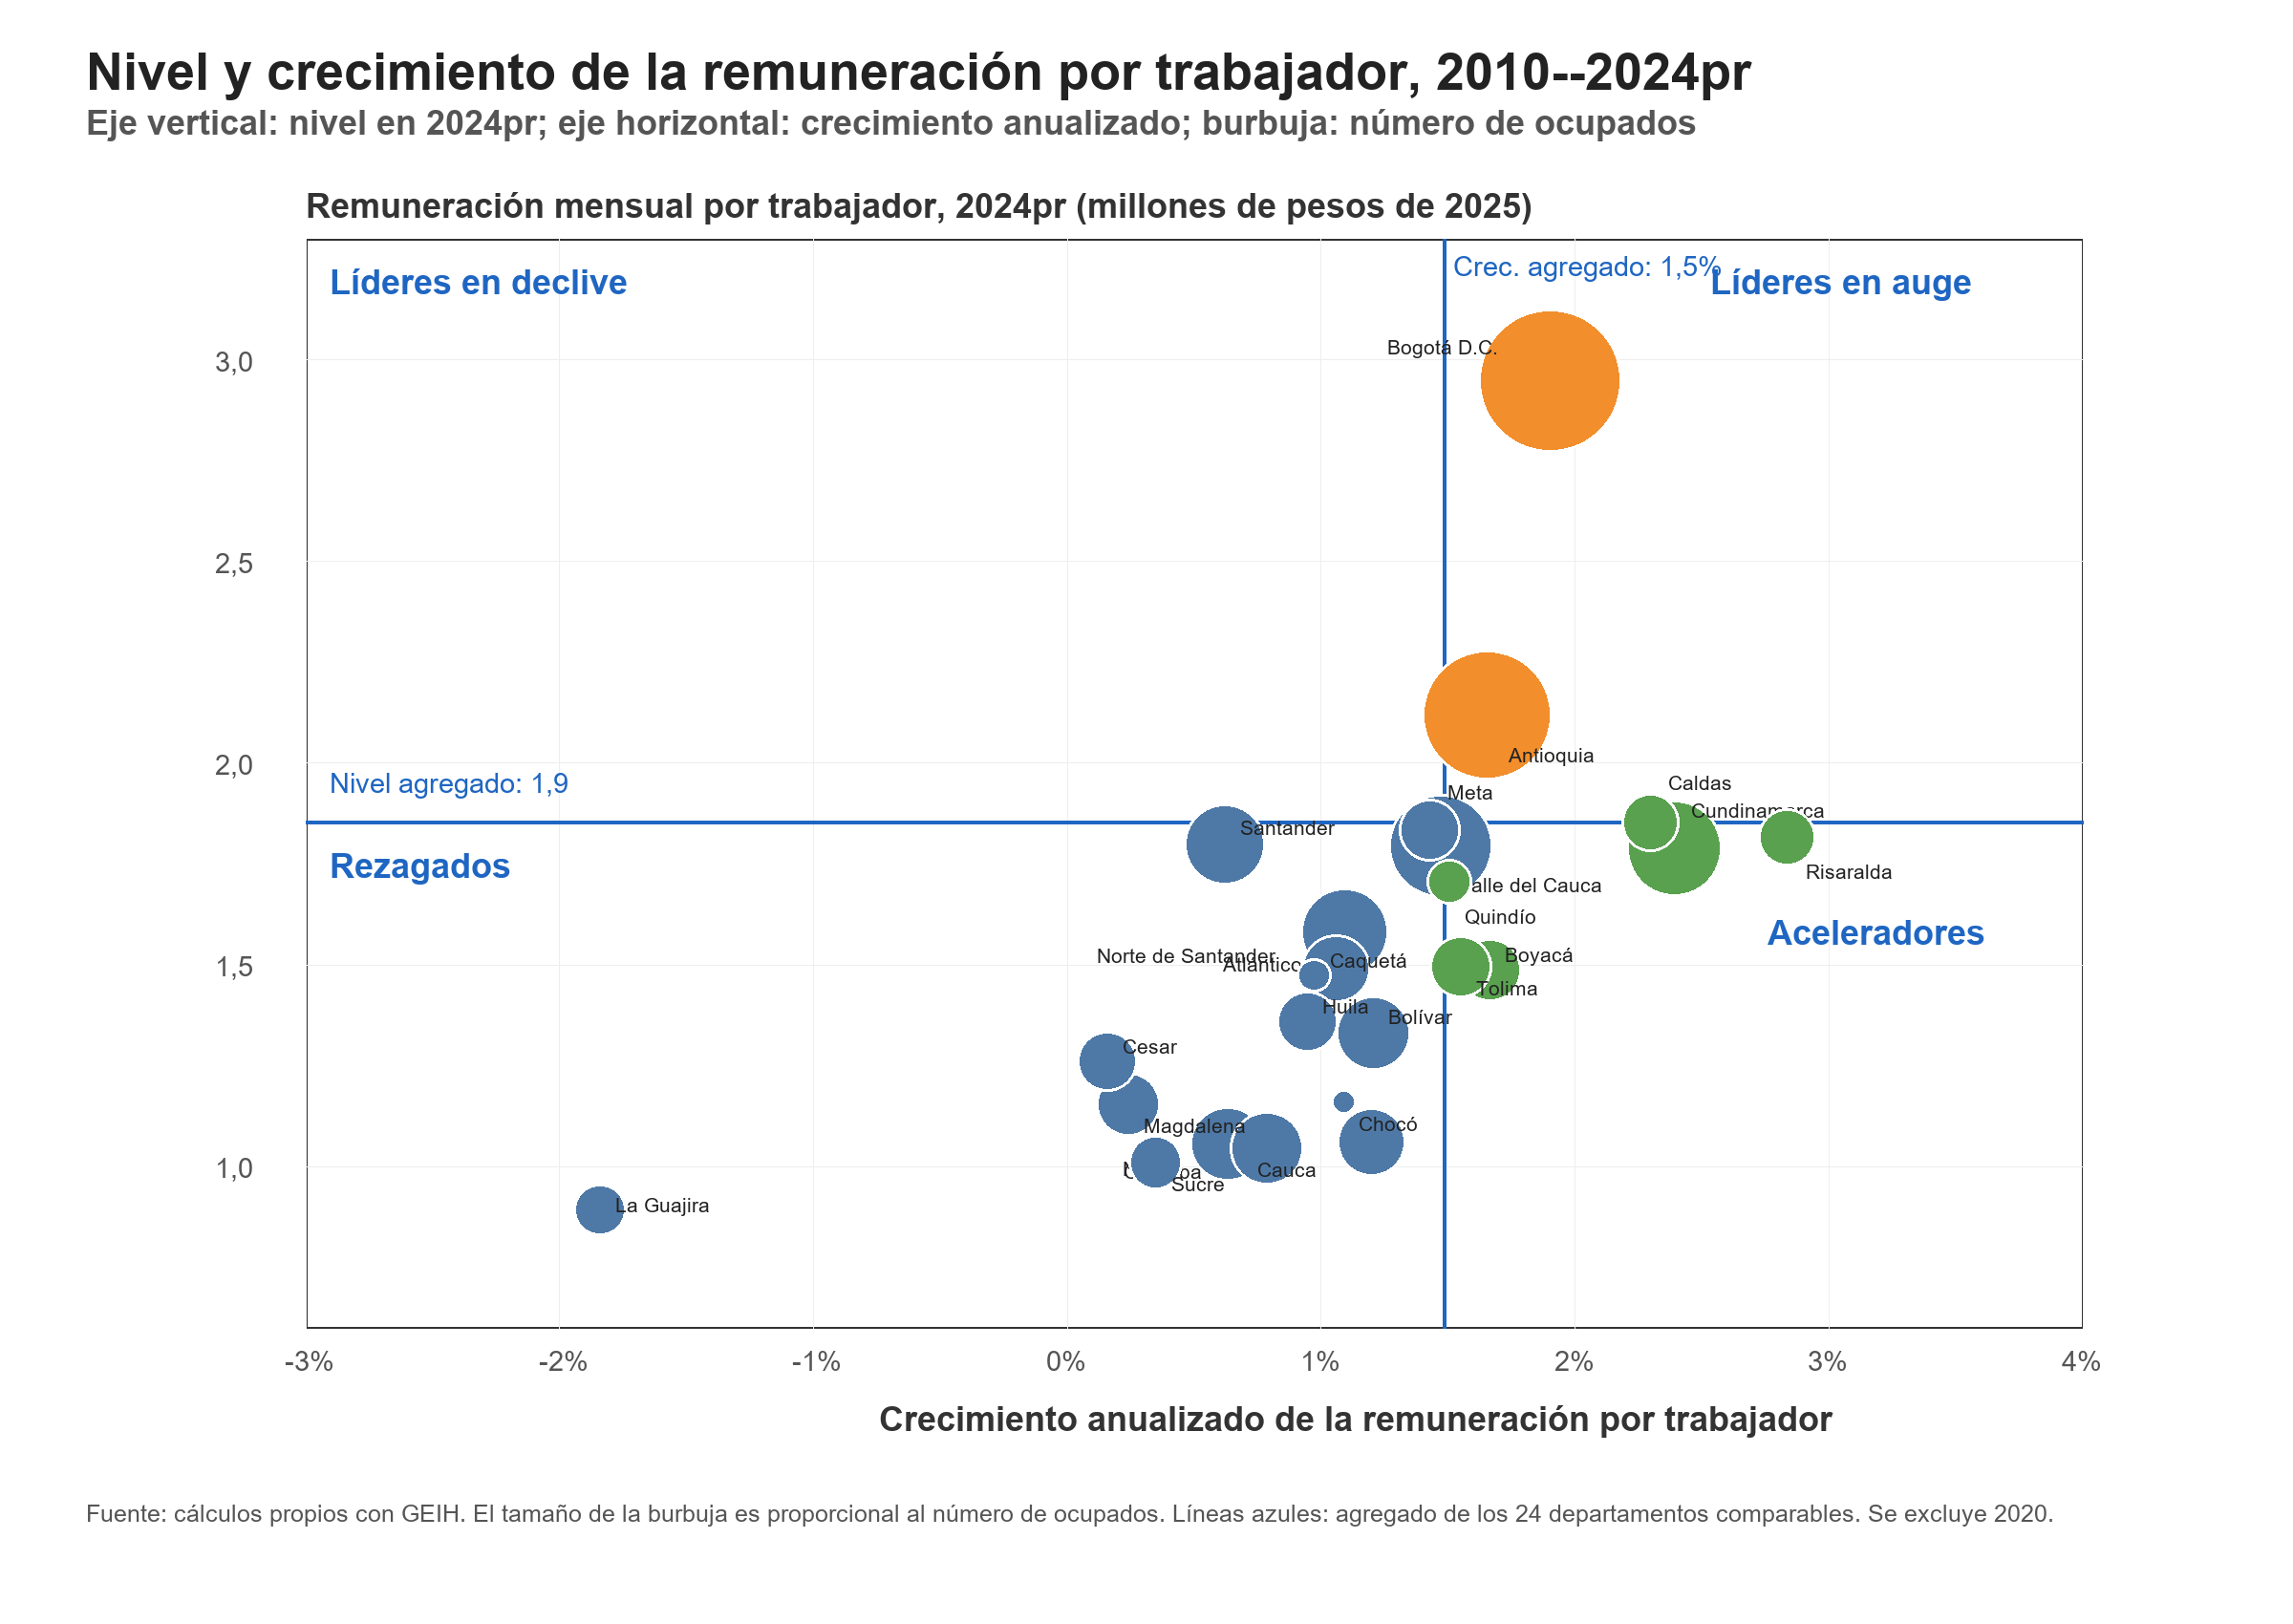
\includegraphics[width=\textwidth]{Paper/figures/fig_geih_remuneracion_departamento_cuadrantes.png}
  \caption{Nivel y crecimiento de la remuneración por trabajador por departamento, 2010--2024pr}
  \label{fig:geih_remuneracion_departamento_cuadrantes}
  \caption*{\footnotesize Nota: la línea vertical muestra el crecimiento agregado de la remuneración por trabajador y la línea horizontal muestra el nivel agregado de remuneración por trabajador en 2024pr. El tamaño de la burbuja es proporcional al número de ocupados del departamento. Fuente: cálculos propios con GEIH.}
\end{figure}

\begin{figure}[H]
  \centering
  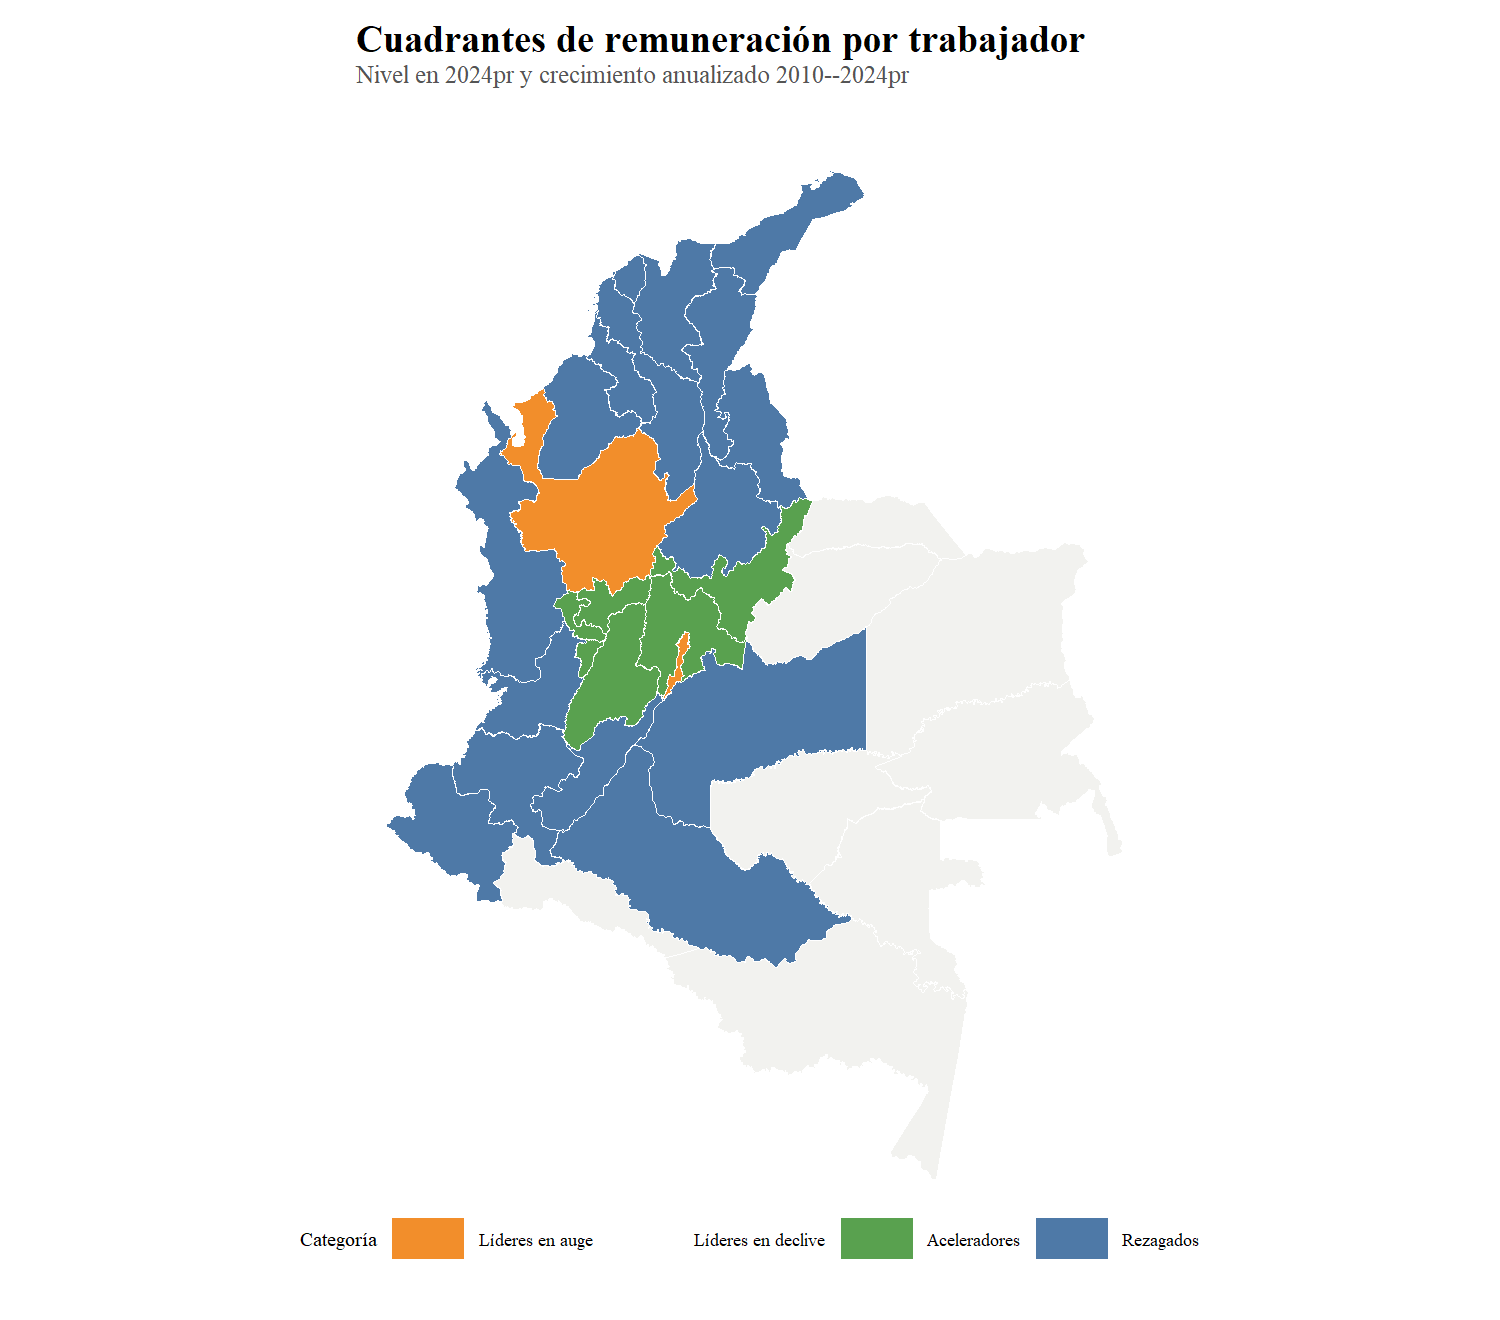
\includegraphics[width=0.82\textwidth]{Paper/figures/fig_geih_remuneracion_departamento_mapa_cuadrantes.png}
  \caption{Mapa de cuadrantes de remuneración por trabajador, 2010--2024pr}
  \label{fig:geih_remuneracion_departamento_mapa_cuadrantes}
  \caption*{\footnotesize Nota: las categorías son las mismas de la Figura \ref{fig:geih_remuneracion_departamento_cuadrantes}. Los departamentos no comparables aparecen en gris. Fuente: cálculos propios con GEIH; geometría departamental de GADM.}
\end{figure}

\textbf{La dinámica de la remuneración laboral tiene una dimensión territorial marcada.} Como muestra la Figura \ref{fig:geih_remuneracion_departamento_mapa_cuadrantes}, buena parte de los departamentos rezagados se ubica en la periferia norte, pacífica y sur del país, mientras que varios de los aceleradores se concentran en el centro andino. Esta distribución sugiere que la relación entre productividad y remuneración no puede separarse de la geografía económica del país.

\section{Conclusiones}

\textbf{Productividad y remuneración están asociadas, pero no se mueven de manera idéntica.} En niveles, los departamentos con mayor PIB por trabajador tienden a tener mayores remuneraciones por trabajador. Sin embargo, la relación no es perfecta y se debilita cuando se comparan las tasas de crecimiento entre 2010 y 2024pr.

\textbf{Los departamentos que se apartan de la relación promedio plantean preguntas importantes.} Bogotá D.C., Caldas, Antioquia, Norte de Santander, Quindío, Caquetá y Risaralda registran remuneraciones superiores a las que sugiere su nivel de PIB por trabajador. Bolívar, Santander, Meta, La Guajira y Boyacá se ubican por debajo de la tendencia. Estos casos deben estudiarse con más detalle, porque pueden reflejar diferencias en composición sectorial, informalidad, estructura empresarial, capital humano y condiciones locales del mercado laboral.

\textbf{Los aumentos de productividad no se traducen automáticamente en aumentos de remuneración.} Quindío y Caquetá registraron crecimientos altos del PIB por trabajador, pero no estuvieron entre los mayores crecimientos de remuneración por trabajador. En cambio, Cundinamarca tuvo un crecimiento relativamente alto de remuneración pese a un desempeño débil del PIB por trabajador. Este desacople muestra que la política pública debe mirar simultáneamente productividad, empleo, formalidad y remuneración.

\textbf{La agenda de productividad necesita una lectura territorial explícita.} Las diferencias entre departamentos no son solo diferencias de nivel; también son diferencias en la forma como la producción se conecta con los ingresos laborales. Por eso, una agenda nacional de productividad debe preguntarse no solo dónde se produce más, sino también dónde esa productividad se transforma en mejores remuneraciones para los trabajadores.
